\section{Experimental Evaluation}
\label{sec:eval}

This section compares APR-BALS with its FP32 baseline in a two-path harness that isolates the precision dispatch. Optimizations that apply to only one path, such as momentum, are evaluated in Section~\ref{sec:extended}.

\subsection{Setup and Methodology}
\label{ssec:setup}

Table~\ref{tab:platforms} lists the platforms and datasets. The primary GPU is an RTX~3060 (Ampere); a Tesla~T4 (Turing), accessed through Google Colab, checks portability. All binaries are built from one source tree with \texttt{nvcc -O3} for \texttt{sm\_86} or \texttt{sm\_75}. We use MovieLens 10M, 20M, and 32M \cite{harper2016movielens} and the Netflix Prize data \cite{bennett2007netflix}, each split once at random into 80\% training and 20\% test ratings. Because the split is random, not the Netflix probe set, absolute RMSE is not comparable with leaderboard results.

\begin{table}[!t]
\caption{Execution Platforms and Datasets. Density Is over All Ratings Before the Split}
\label{tab:platforms}
\centering
\footnotesize
\renewcommand{\arraystretch}{1.05}
\setlength{\tabcolsep}{3pt}
\begin{tabular}{lcc}
\toprule
 & \textbf{RTX 3060} & \textbf{Tesla T4} \\
\midrule
Architecture & Ampere, sm\_86 & Turing, sm\_75 \\
SMs, memory & 28, 12 GB & 40, 16 GB \\
FP32 peak (TFLOP/s) & 12.7 & 8.1 \\
FP16 tensor, FP32 acc.\ (TFLOP/s) & 25.5 & 65 \\
CUDA & 12.0, 12.9 & 12 (Colab) \\
\bottomrule
\end{tabular}

\vspace{4pt}

\setlength{\tabcolsep}{2.5pt}
\begin{tabular}{lrrrrr}
\toprule
\textbf{Dataset} & \textbf{Users} & \textbf{Items} & \textbf{Train} & \textbf{Test} & \textbf{Density} \\
\midrule
ML-10M   & 69{,}878  & 10{,}677 & 8{,}026{,}731  & 1{,}973{,}323 & 1.3\% \\
ML-20M   & 138{,}493 & 26{,}744 & 16{,}052{,}927 & 3{,}947{,}336 & 0.54\% \\
ML-32M   & 200{,}948 & 84{,}432 & 25{,}677{,}530 & 6{,}322{,}674 & 0.19\% \\
Netflix  & 480{,}189 & 17{,}770 & 80{,}570{,}989 & 19{,}909{,}518 & 1.2\% \\
\bottomrule
\end{tabular}
\end{table}

Accuracy is the root-mean-square error on the held-out test ratings, and the cost of mixed precision is the relative difference $\Delta = |\mathrm{RMSE}_{\mathrm{APR}} - \mathrm{RMSE}_{\mathrm{base}}| / \mathrm{RMSE}_{\mathrm{base}}$. Speed is reported as the \textit{wall-time speedup}, the ratio of training-loop times from the first sweep to convergence, including RMSE checks. One-time preprocessing, tile construction, and host-to-device transfers, which both paths share, are excluded. Times come from CUDA events on an otherwise idle GPU, and per-stage times from events around every batch.

\textbf{Measurement variability.} Every configuration in Table~\ref{tab:main3060} was run five times in one session, 100 runs in total. The relative standard deviation of the wall-time speedup is at most $0.44\%$ (mean $0.14\%$), and every tabulated speedup reproduces within $0.50\%$. We therefore treat differences below $1\%$ as insignificant. Test RMSE varies by at most $10^{-6}$ across the same runs.

\subsection{Speedup and Accuracy}
\label{ssec:main_results}

Table~\ref{tab:main3060} and Fig.~\ref{fig:speedup_vs_k}(a) report the RTX~3060 results. The baseline and APR-BALS stop after the same number of sweeps in every configuration, so mixed precision does not alter the optimization trajectory. The speedup grows with $K$ because tensor-core efficiency improves with operand width while the scalar baseline's throughput stays nearly flat. On Netflix it rises from $4.07\times$ at $K=16$ to $14.84\times$ at $K=96$. The MovieLens datasets peak at $K=64$ ($11.62\times$ on ML-20M, $11.59\times$ on ML-32M, $10.87\times$ on ML-10M). This peak is real: on ML-20M the $K=64$ and $K=96$ speedups differ by $4.1\%$, ten times the measurement variability.

\begin{table}[!t]
\caption{FP32 Baseline Versus APR-BALS on the RTX 3060. Both Paths Stop After the Same Number of Sweeps (20 on Netflix, 25 on MovieLens). $\Delta$ Is the Relative Test-RMSE Difference in Units of $10^{-3}\%$; APR-BALS Has the Lower RMSE at Every Point. Over Five Repeated Runs, the Relative Standard Deviation of Every Speedup Is at Most $0.44\%$}
\label{tab:main3060}
\centering
\footnotesize
\renewcommand{\arraystretch}{1.02}
\setlength{\tabcolsep}{3.5pt}
\begin{tabular}{llrrrrr}
\toprule
\textbf{Dataset} & & \textbf{$K{=}16$} & \textbf{32} & \textbf{48} & \textbf{64} & \textbf{96} \\
\midrule
\multirow{4}{*}{Netflix}
 & base (s)       & 4.83 & 14.39 & 31.76 & 74.18 & 154.42 \\
 & APR (s)        & 1.19 & 2.00 & 3.13 & 5.34 & 10.41 \\
 & speedup        & 4.07 & 7.21 & 10.14 & 13.90 & \textbf{14.84} \\
 & $\Delta$       & 2.9 & 3.2 & 3.8 & 4.0 & 4.3 \\
\midrule
\multirow{4}{*}{ML-32M}
 & base (s)       & 2.40 & 6.95 & 15.34 & 35.22 & 78.80 \\
 & APR (s)        & 0.54 & 1.00 & 1.69 & 3.04 & 7.28 \\
 & speedup        & 4.43 & 6.94 & 9.07 & \textbf{11.59} & 10.82 \\
 & $\Delta$       & 1.1 & 1.5 & 1.6 & 1.7 & 1.8 \\
\midrule
\multirow{4}{*}{ML-20M}
 & base (s)       & 1.23 & 3.65 & 7.92 & 18.60 & 39.95 \\
 & APR (s)        & 0.30 & 0.54 & 0.90 & 1.60 & 3.58 \\
 & speedup        & 4.08 & 6.76 & 8.83 & \textbf{11.62} & 11.16 \\
 & $\Delta$       & 0.8 & 0.9 & 1.2 & 1.2 & 1.3 \\
\midrule
\multirow{4}{*}{ML-10M}
 & base (s)       & 0.52 & 1.60 & 3.40 & 8.13 & 16.84 \\
 & APR (s)        & 0.13 & 0.25 & 0.42 & 0.75 & 1.61 \\
 & speedup        & 3.93 & 6.42 & 8.16 & \textbf{10.87} & 10.45 \\
 & $\Delta$       & 0.5 & 0.5 & 0.6 & 0.5 & 0.6 \\
\bottomrule
\end{tabular}
\end{table}

\begin{figure}[!t]
\centering
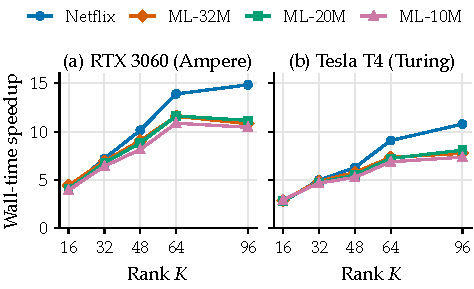
\includegraphics[width=\columnwidth]{figures/fig_speedup.pdf}
\caption{Wall-time speedup of APR-BALS over the FP32 baseline versus latent dimension. }
\label{fig:speedup_vs_k}
\end{figure}

The test-RMSE difference never exceeds $0.0043\%$, and APR-BALS has the lower error at all 20 points. It also has the lower training error, so the effect is not FP16 rounding acting as a regularizer; we have not isolated its cause. The difference grows slowly with $K$ (Netflix: $0.0029\%$ to $0.0043\%$), consistent with the degree-independent error term of \eqref{eq:error_bound}. For scale, raising $K$ from 64 to 96 improves the Netflix test RMSE by $0.19\%$, which is $44$ times larger than the largest precision effect. Test RMSE improves monotonically with $K$ on every dataset, so the most accurate configuration is also the fastest.
\subsection{Cross-Architecture Reproduction}
\label{ssec:t4}

On the Tesla~T4 (Fig.~\ref{fig:speedup_vs_k}(b), single runs, same source and protocol) the speedup is lower but grows with $K$ in the same way, reaching $10.78\times$ on Netflix at $K=96$. The T4's tensor-to-FP32 peak ratio is eight times the RTX~3060's, so peak ratios do not predict the gain of these staging-bound kernels. Accuracy differences stay below $0.007\%$.

\subsection{Where the Time Goes}
\label{ssec:analysis}

Fig.~\ref{fig:stages} breaks the Netflix runs into stages. The baseline's Gram stage sustains 187--280~GFLOP/s, about $2\%$ of FP32 peak, as expected for gather-bound sparse work. APR-BALS raises the same stage to 1.0--11.5~TFLOP/s (both upper bounds). The item side reaches the higher rates because items average more ratings than users, which gives the WMMA kernels longer accumulation loops. Fig.~\ref{fig:stages}(b) shows the consequence. The Gram stage takes 89--96\% of a baseline sweep but only 38--56\% of an APR-BALS sweep, and at $K=96$ the solve becomes the largest stage (48\%), which is why Section~\ref{sec:extended} turns to the solver.

\begin{figure}[!t]
\centering
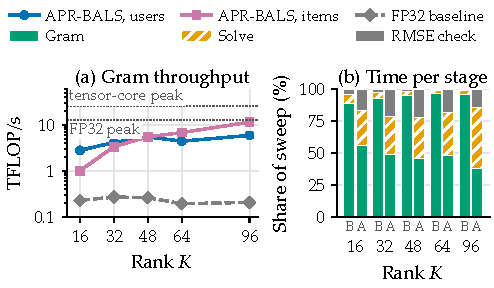
\includegraphics[width=\columnwidth]{figures/fig_stages.pdf}
\caption{Per-stage profile of the Netflix runs on the RTX~3060, both paths of the two-path harness. (a) Gram-stage throughput of APR-BALS per side and of the FP32 baseline (both sides combined), against the peaks of Table~\ref{tab:platforms}. (b) Share of sweep time per stage; under each $K$, bar B is the FP32 baseline and bar A is APR-BALS. Gram time is exposed time, the stage span minus the busy time of the solve that overlaps it, so the throughput in (a) is an upper bound.}
\label{fig:stages}
\end{figure}

\textbf{What limits the tensor-core kernels.} Table~\ref{tab:ncu} lists Nsight Compute counters for the shipped configuration at $K=96$. The dense WMMA kernel uses only $20.5\%$ of the tensor pipe, so it is not bound by tensor throughput. Its most utilized resource is DRAM ($47.6\%$), about twice its SM throughput, which identifies feature-row staging as the limiter. The giant kernel shows the opposite profile ($75.1\%$ SM, $11.4\%$ DRAM), which supports dispatching the two tiers to separate kernels. Their $16\%$ occupancy is deliberate: 240 registers per thread at $K=96$ allow two blocks per SM, and the measured $16.0\%$ matches the predicted $16.7\%$.

\begin{table}[!t]
\caption{Nsight Compute Counters, Netflix $K=96$, RTX 3060. One Steady-State Launch per Kernel; Values Are Percentages of Peak. ``Theor.'' Is the Occupancy Limit Implied by Register Use}
\label{tab:ncu}
\centering
\footnotesize
\renewcommand{\arraystretch}{1.05}
\setlength{\tabcolsep}{2.5pt}
\begin{tabular}{lrrrrrr}
\toprule
 & \textbf{Tensor} & \multicolumn{2}{c}{\textbf{Occupancy}} & & & \\
\textbf{Kernel} & \textbf{pipe} & \textbf{ach.} & \textbf{theor.} & \textbf{SM} & \textbf{DRAM} & \textbf{Regs} \\
\midrule
Dense WMMA Gram       & 20.5 & 16.0 & 16.7 & 25.5 & \textbf{47.6} & 240 \\
Giant WMMA Gram       & 24.3 & 16.6 & 16.7 & \textbf{75.1} & 11.4 & 255 \\
Sparse scalar Gram    & 0.0  & 69.1 & ---  & 29.7 & 42.2 & 64 \\
Cholesky, FP16 tiles  & 0.0  & 54.5 & ---  & 58.4 & 11.0 & 40 \\
\bottomrule
\end{tabular}
\end{table}

\textbf{The solve as the second bottleneck.} In the baseline the solve takes less than $3\%$ of a sweep; in APR-BALS it takes $33$--$41\%$ of the Gram-plus-solve time at $K=16$--$64$ and $56\%$ at $K=96$, and without the blocked solver the $K \ge 48$ speedups would be $28$--$41\%$ lower. The solver is now near a structural floor, launching only $0.96$ waves per SM at $K=96$. A timeline of the shipped binary confirms that the GPU is busy for $99.6\%$ of the run and that the scalar tier accounts for at most $3.2\%$ of wall time, so further gains must come from faster kernels rather than better scheduling.

\subsection{WMMA Kernel Versus Reduced Precision}
\label{ssec:precisioniso}

The two-path comparison changes two things at once: the execution unit and the operand precision. Ampere allows the two to be separated, because WMMA also accepts TF32 operands, which keep the full FP32 exponent range and have eight more mantissa bits than FP16. We built three variants of the Gram stage in one binary, differing by a single compile flag each: the shipped FP16 kernel (\texttt{HMMA.16816.F32}), a TF32 kernel on the same tensor pipe (\texttt{HMMA.1684.F32.TF32}), and the scalar FP32 kernel, selected by raising $\theta_d$ above every entity's degree. Solver, batching, convergence rule, and data are identical. FP16 and TF32 share one dataflow, so their ratio isolates precision. The scalar kernel differs in dataflow as well as execution unit (tiles, full $K \times K$ output, atomic flushes), so its ratio to TF32 measures the WMMA kernel design as a whole; an FP32 CUDA-core kernel with the WMMA dataflow was not built. The giant tier is disabled in all three, because a TF32 giant kernel would exceed the 48~KB static shared-memory limit. The TF32 kernel is inert when disabled; the unmodified build's disassembly is byte-identical.

\begin{table}[!t]
\caption{Precision-Isolating Ablation, Netflix, RTX 3060, Giant Tier Disabled. Milliseconds per Sweep of the Gram Stage Together with the Solve That Overlaps It (Identical in All Three), and the Split of the Total Speedup into a Kernel Factor (FP32 Scalar over TF32) and a Precision Factor (TF32 over FP16). ``Share'' Is $\ln(\text{kernel})/\ln(\text{total})$. All Runs Take 20 Sweeps}
\label{tab:precisioniso}
\centering
\footnotesize
\renewcommand{\arraystretch}{1.05}
\setlength{\tabcolsep}{3pt}
\begin{tabular}{crrrrrr}
\toprule
 & \multicolumn{3}{c}{\textbf{Gram + solve (ms)}} & \multicolumn{3}{c}{\textbf{Decomposition}} \\
\textbf{$K$} & \textbf{FP16} & \textbf{TF32} & \textbf{FP32} & \textbf{Kernel} & \textbf{Prec.} & \textbf{Share} \\
\midrule
16 & 44.4  & 54.3  & 231.4   & 4.26$\times$  & 1.22$\times$ & 87.8\% \\
32 & 70.2  & 82.5  & 695.0   & 8.42$\times$  & 1.18$\times$ & 92.9\% \\
48 & 106.8 & 141.2 & 1549.7  & 10.98$\times$ & 1.32$\times$ & 89.6\% \\
64 & 209.5 & 212.2 & 3647.1  & 17.19$\times$ & 1.01$\times$ & \textbf{99.6\%} \\
96 & 428.8 & 484.7 & 7624.1  & 15.73$\times$ & 1.13$\times$ & 95.7\% \\
\bottomrule
\end{tabular}
\end{table}

Table~\ref{tab:precisioniso} shows that the WMMA kernel, not the reduced precision, produces the gain. At full FP32 range, the TF32 kernel is already $4.3$--$17.2\times$ faster than the scalar kernel, which is $87.8$--$99.6\%$ of the total effect. Moving from TF32 to FP16 adds at most $1.32\times$, and nothing measurable at $K=64$. On ML-20M and ML-10M at $K \in \{32, 96\}$ the kernel share is $92.2$--$96.7\%$, so the result is not specific to Netflix. The small precision factor also confirms the roofline reading: Ampere's TF32 tensor peak is half the FP16 rate, about the FP32 CUDA-core peak, so a throughput-bound kernel would lose about $2\times$, whereas this one loses at most $1.32\times$. For the same reason the $4$--$17\times$ kernel factor cannot come from peak arithmetic rate; it comes from the WMMA kernels' register accumulation, atomic-free output, and triangular work. Accuracy follows the order TF32 $\le$ FP16 $<$ scalar FP32 at every rank, with a total spread of $0.018\%$. Because the measured phase includes the identical solve, every ratio understates the Gram-only effect.

\subsection{Sensitivity and Reproducibility}
\label{ssec:sensitivity}

\textbf{Tier thresholds.} Both thresholds were swept on Netflix at $K=96$ with the shipped binary. The giant threshold is forgiving: over $\theta_g \in \{128, \dots, 2048\}$, a sixteen-fold range that moves between 455 and about 97{,}000 users into the giant tier, wall time varies by only $2.7\%$, and 1024 is the measured optimum. The dense threshold is not. Raising $\theta_d$ from 4 to 8, 16, and 32 increases wall time by $1.05\times$, $1.31\times$, and $2.04\times$, because it moves entities from the tensor cores to the scalar tier. Test RMSE is identical to six decimals and all runs take 20 sweeps. The FP16 staging threshold inside the scalar kernel was not swept.

\textbf{Trajectories and determinism.} On Netflix at $K=32$, the two paths' train RMSE agrees to the fourth or fifth decimal at every checkpoint. The baseline is bit-stable across runs. APR-BALS varies in the sixth decimal because the sparse tail's atomic additions complete in a data-dependent order; the WMMA tiers are deterministic.
